\chapter{Complete MySQL Script}
The complete script is supplied as a separate file with this report: \textbf{\texttt{docs/report/hospital\_db\_full.sql}}
(about 130 KB). It was exported with \texttt{mysqldump} from a database built from \texttt{database/seed.sql} and
migrations 000--023, the same schema as \texttt{hospital\_db}, and contains, in order:
\begin{itemize}
\item \texttt{CREATE DATABASE hospital\_db} (utf8mb4) and \texttt{USE hospital\_db};
\item the 33 \texttt{CREATE TABLE} statements with every primary key, foreign key (including the 15 composite consistency keys), UNIQUE key, CHECK constraint, index and the generated column;
\item the sample data as \texttt{INSERT} statements (all people in it are made up; account passwords are bcrypt hashes of the documented demo password);
\item the 10 views, 7 triggers and 5 stored procedures.
\end{itemize}
Load it with \texttt{mysql -u root -p < hospital\_db\_full.sql}. Loaded into an empty server, it produced a database
whose structure matched \texttt{hospital\_db} exactly (schema-diff: no differences). The queries of Section~8.6 are in
\texttt{docs/report/generated/q1.sql} to \texttt{q15.sql}, and the migrations that build the schema step by step are in
\texttt{database/migrations/}.

\chapter{Source Code}
The source code is in the GitHub repository
\textbf{\url{https://github.com/rohithsaivemuri-sudo/hospital-dashboard}} (branch \texttt{main}):
\begin{itemize}
\item \texttt{server/}: the Express API (routes, controllers, services, middleware), migration and test scripts, and the automated tests (\texttt{server/tests});
\item \texttt{client/}: the React application (\texttt{client/src/pages} has one folder per module);
\item \texttt{database/}: the migrations and the seed data;
\item \texttt{tests/ui/}: the browser tests; \texttt{deploy/azure/}: deployment scripts;
\item \texttt{docs/}: this report and its source (\texttt{docs/report}), the BCNF analysis, the database report and the editable ER diagrams (\texttt{er-diagrams.drawio}).
\end{itemize}
A demonstration copy runs at \url{https://hms-demo-in.indonesiacentral.cloudapp.azure.com} (sign-in required).

\chapter{Additional Screenshots}
\begin{figure}[H]\centering
\begin{tabular}{@{}cc@{}}
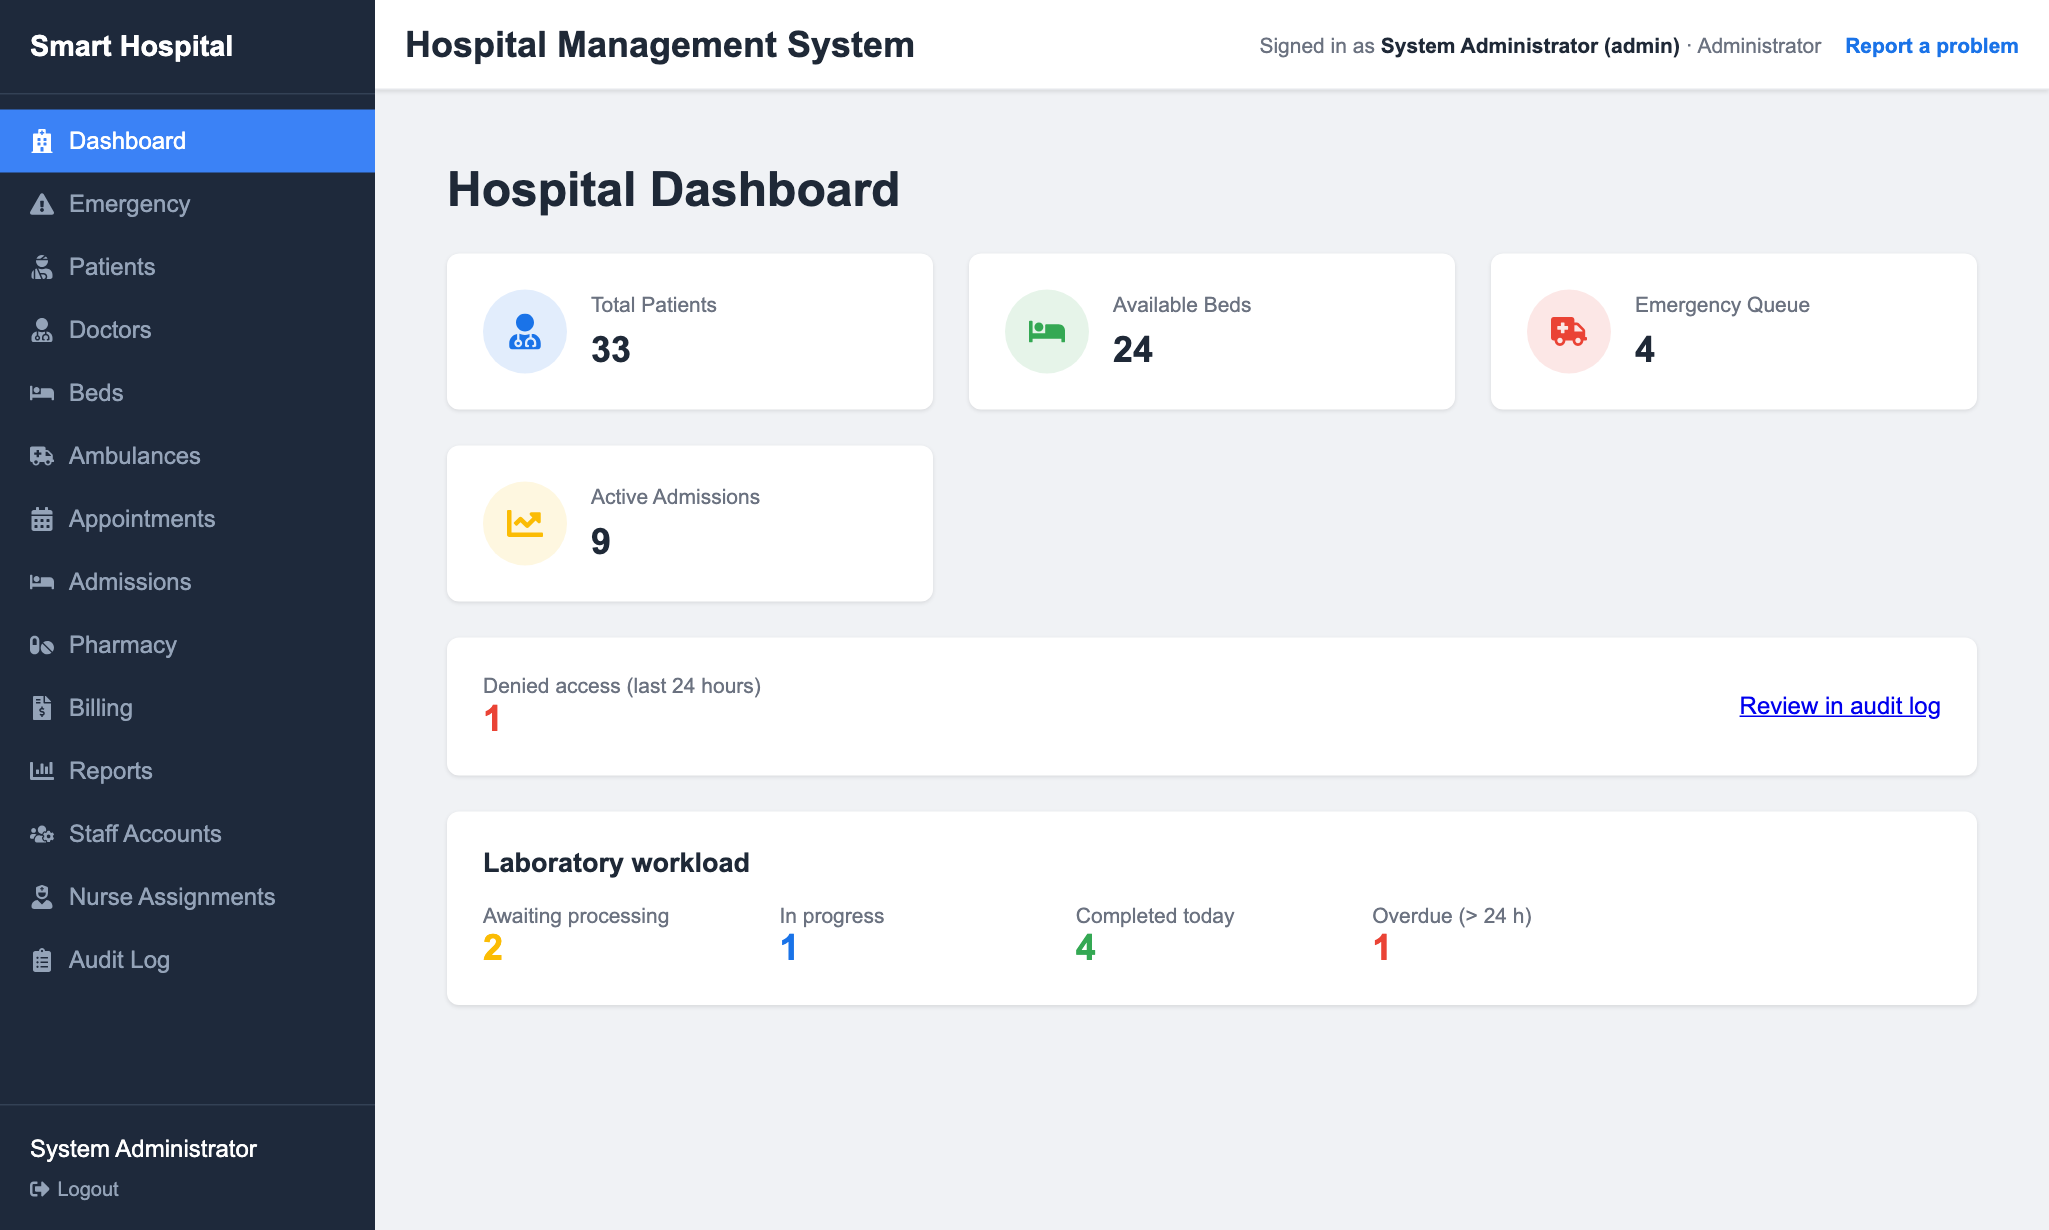
\includegraphics[width=0.485\textwidth]{admin-dashboard.png} & 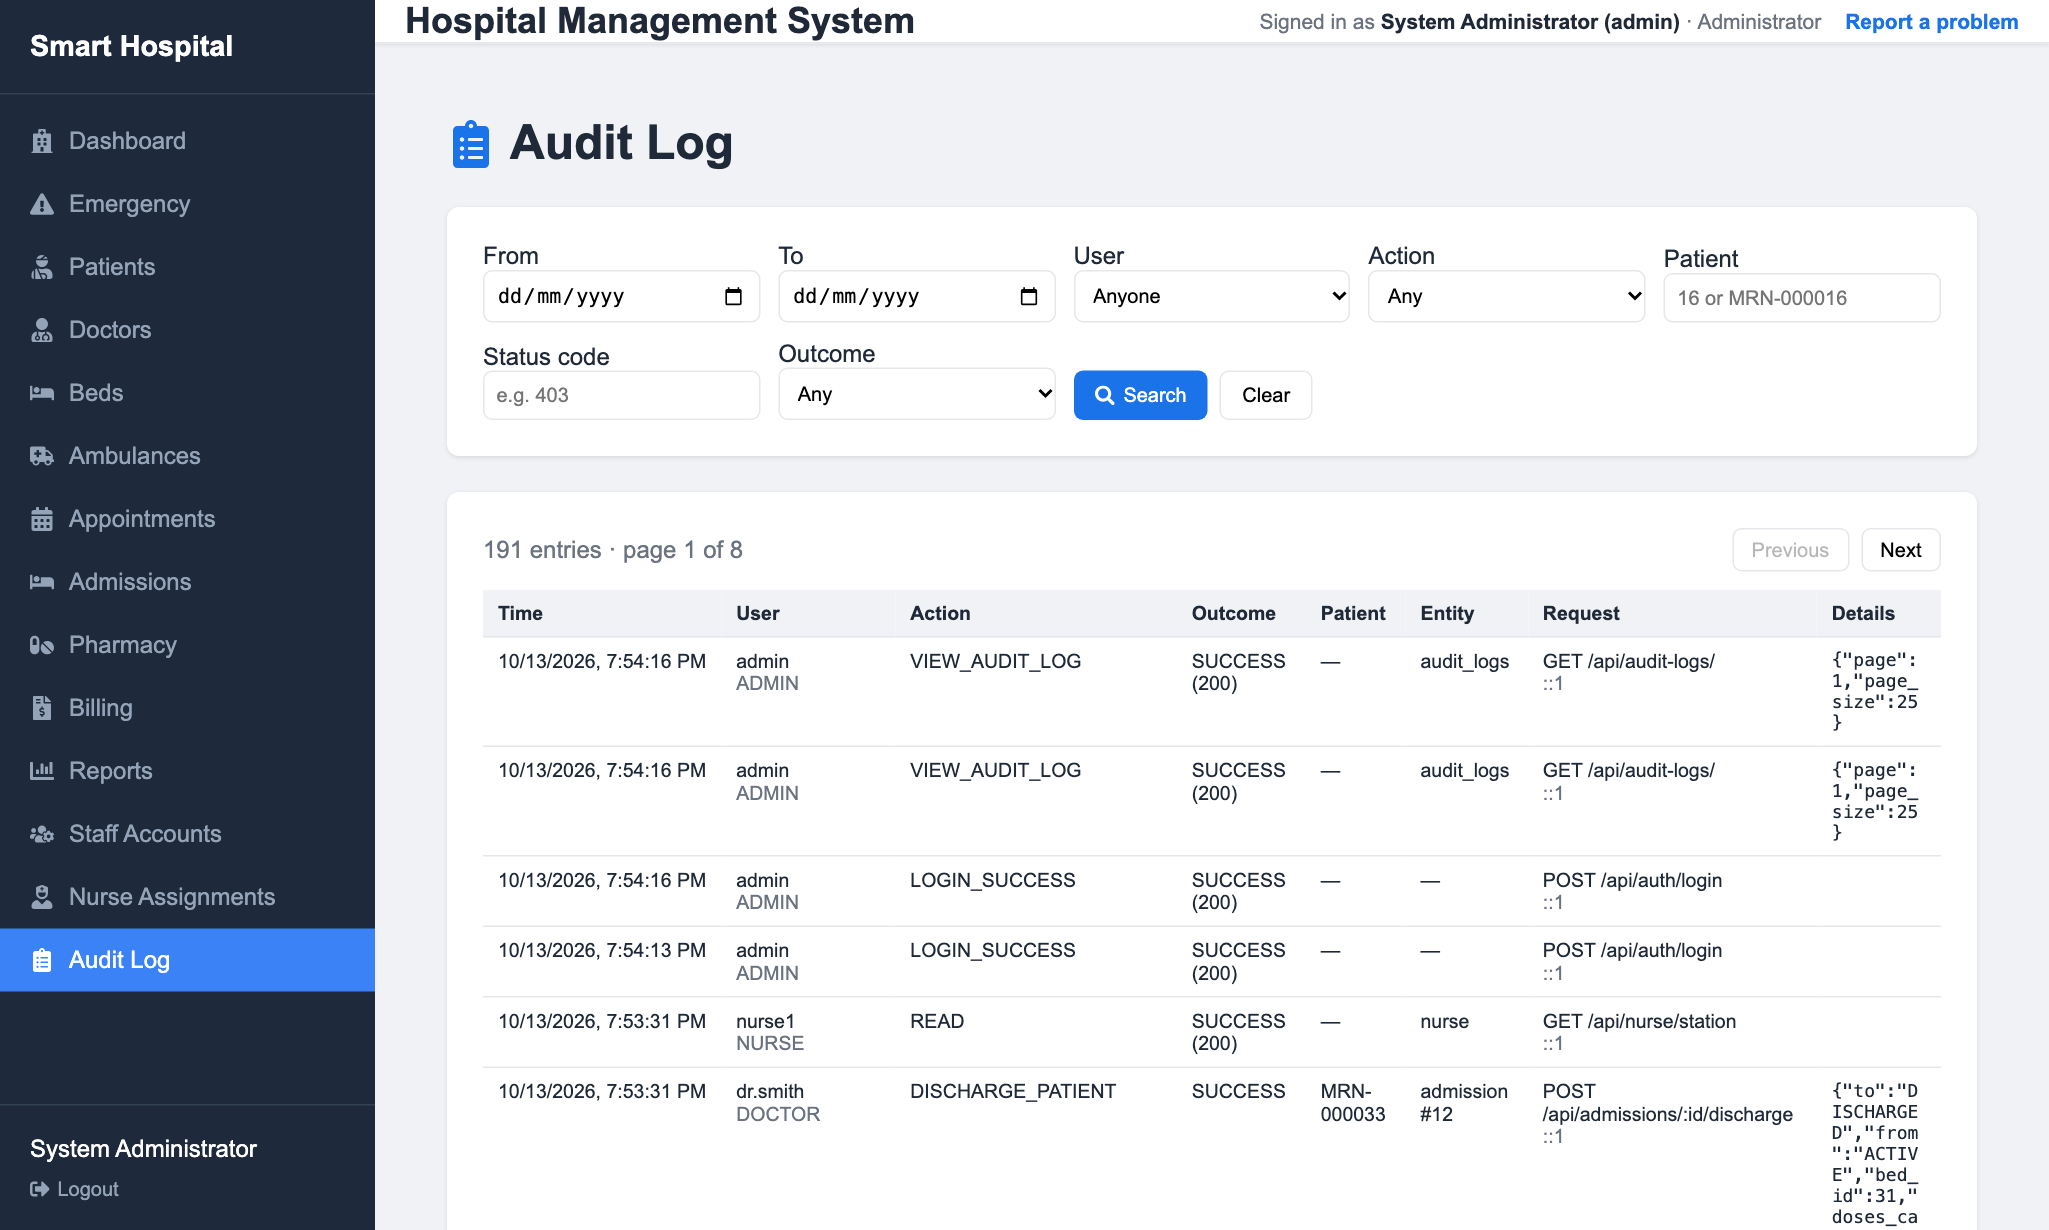
\includegraphics[width=0.485\textwidth]{admin-audit.png} \\
\small (a) Administrator: hospital dashboard & \small (b) Administrator: audit log \\[3pt]
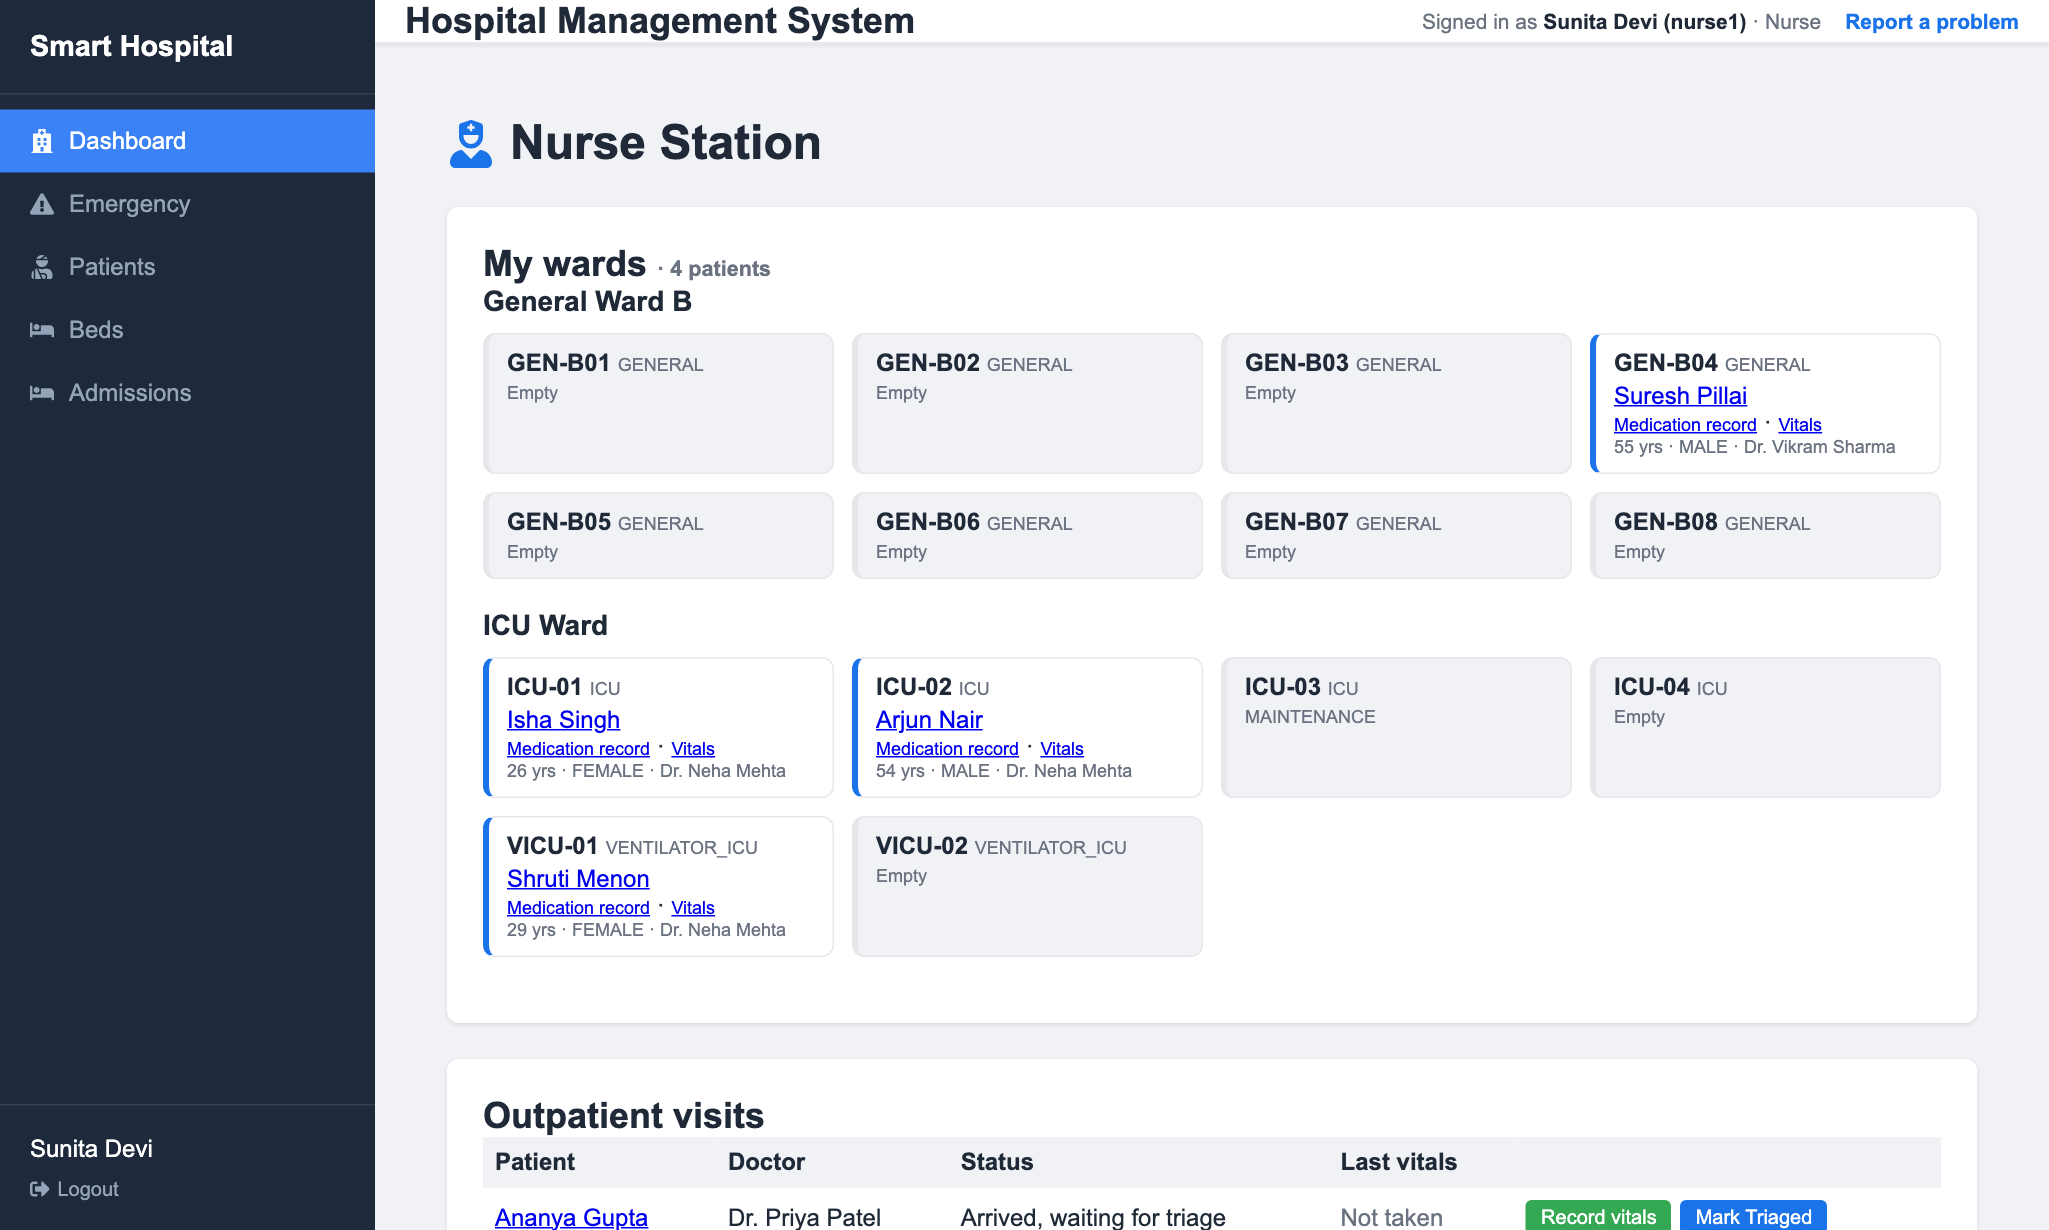
\includegraphics[width=0.485\textwidth]{nurse-station.png} & 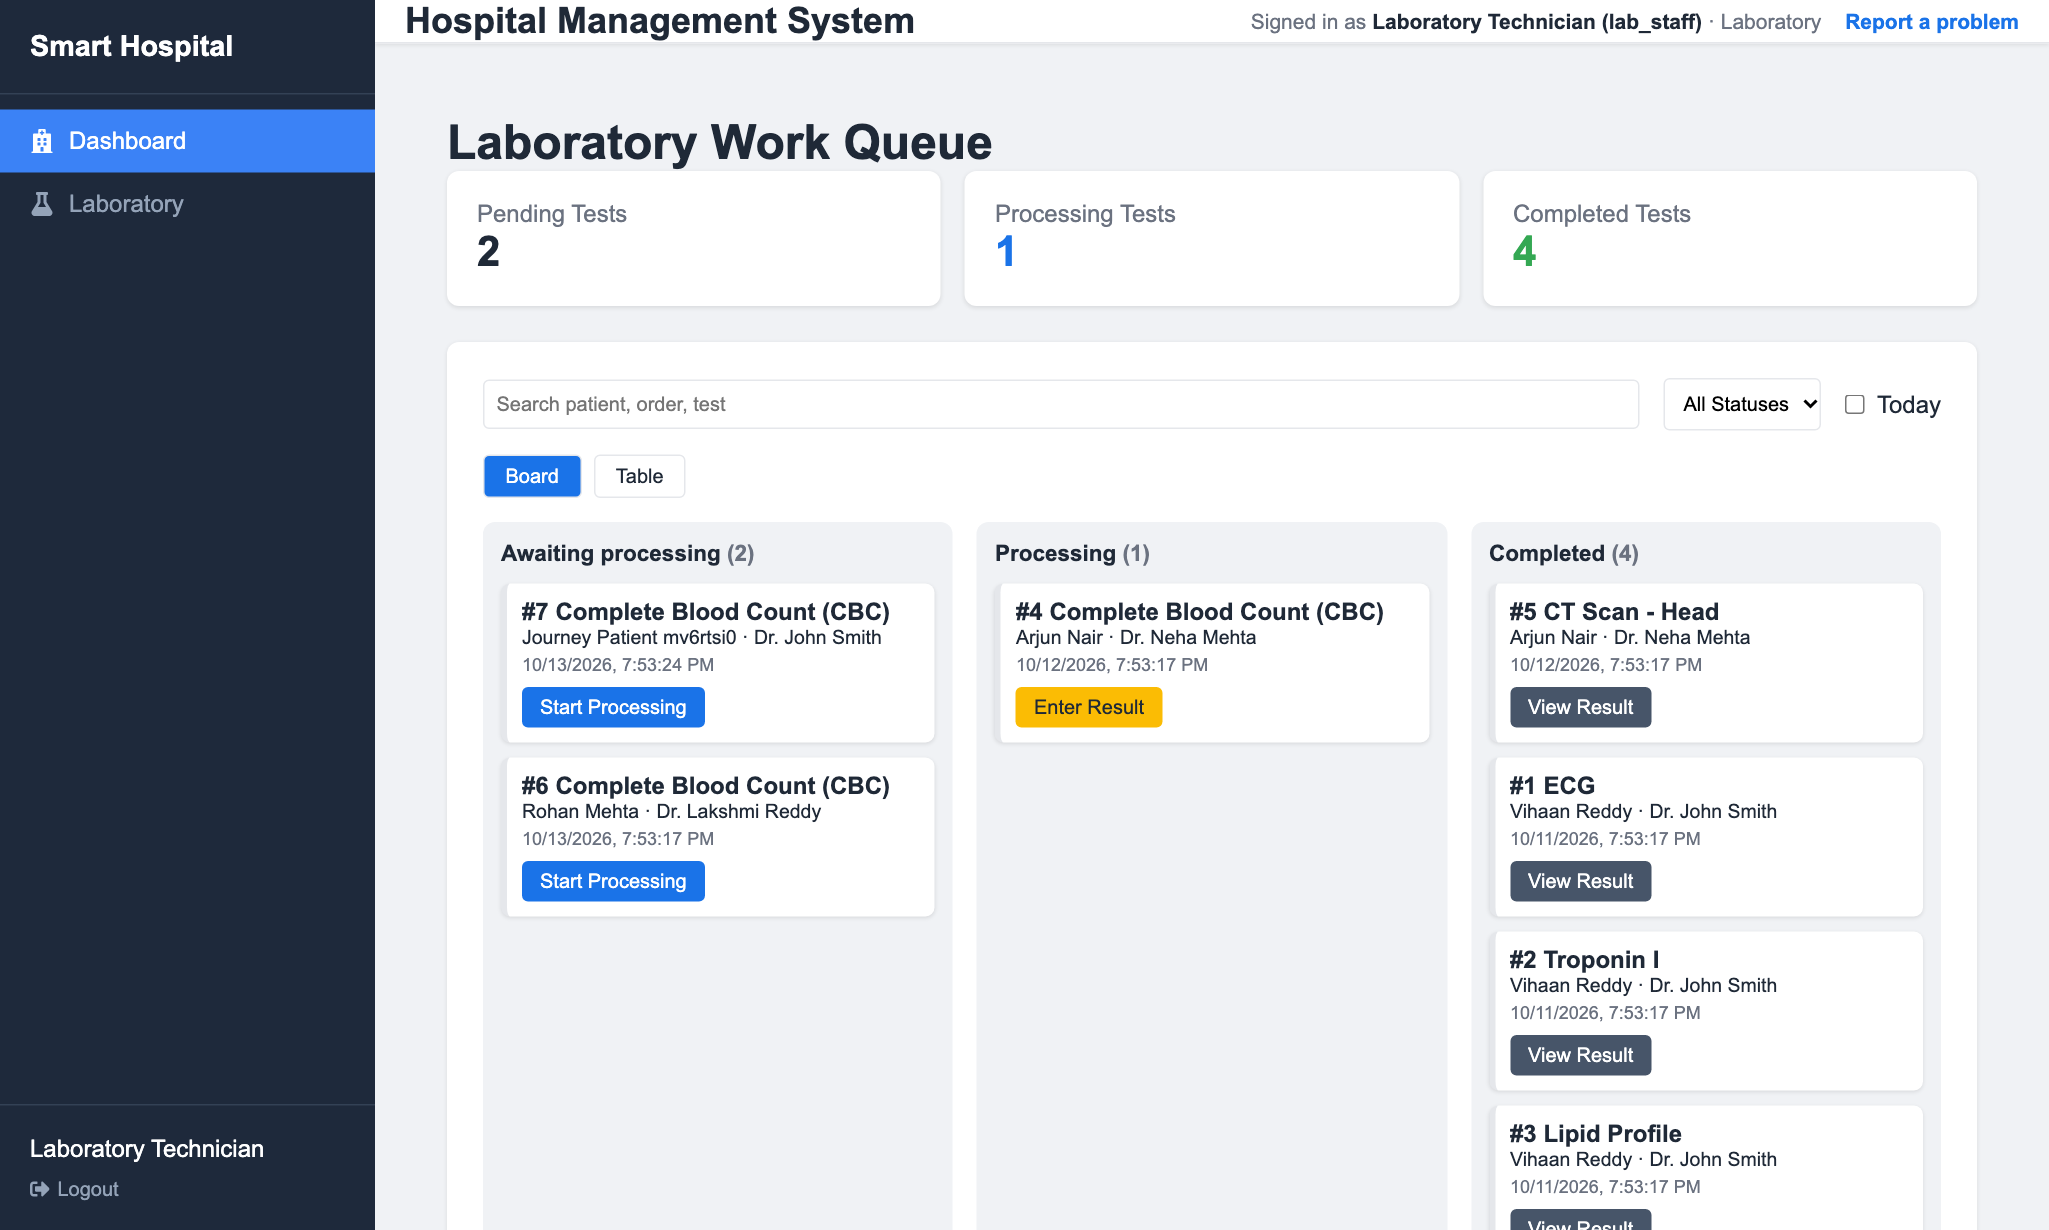
\includegraphics[width=0.485\textwidth]{lab-dashboard.png} \\
\small (c) Nurse: ward station with assigned beds & \small (d) Laboratory: order board \\[3pt]
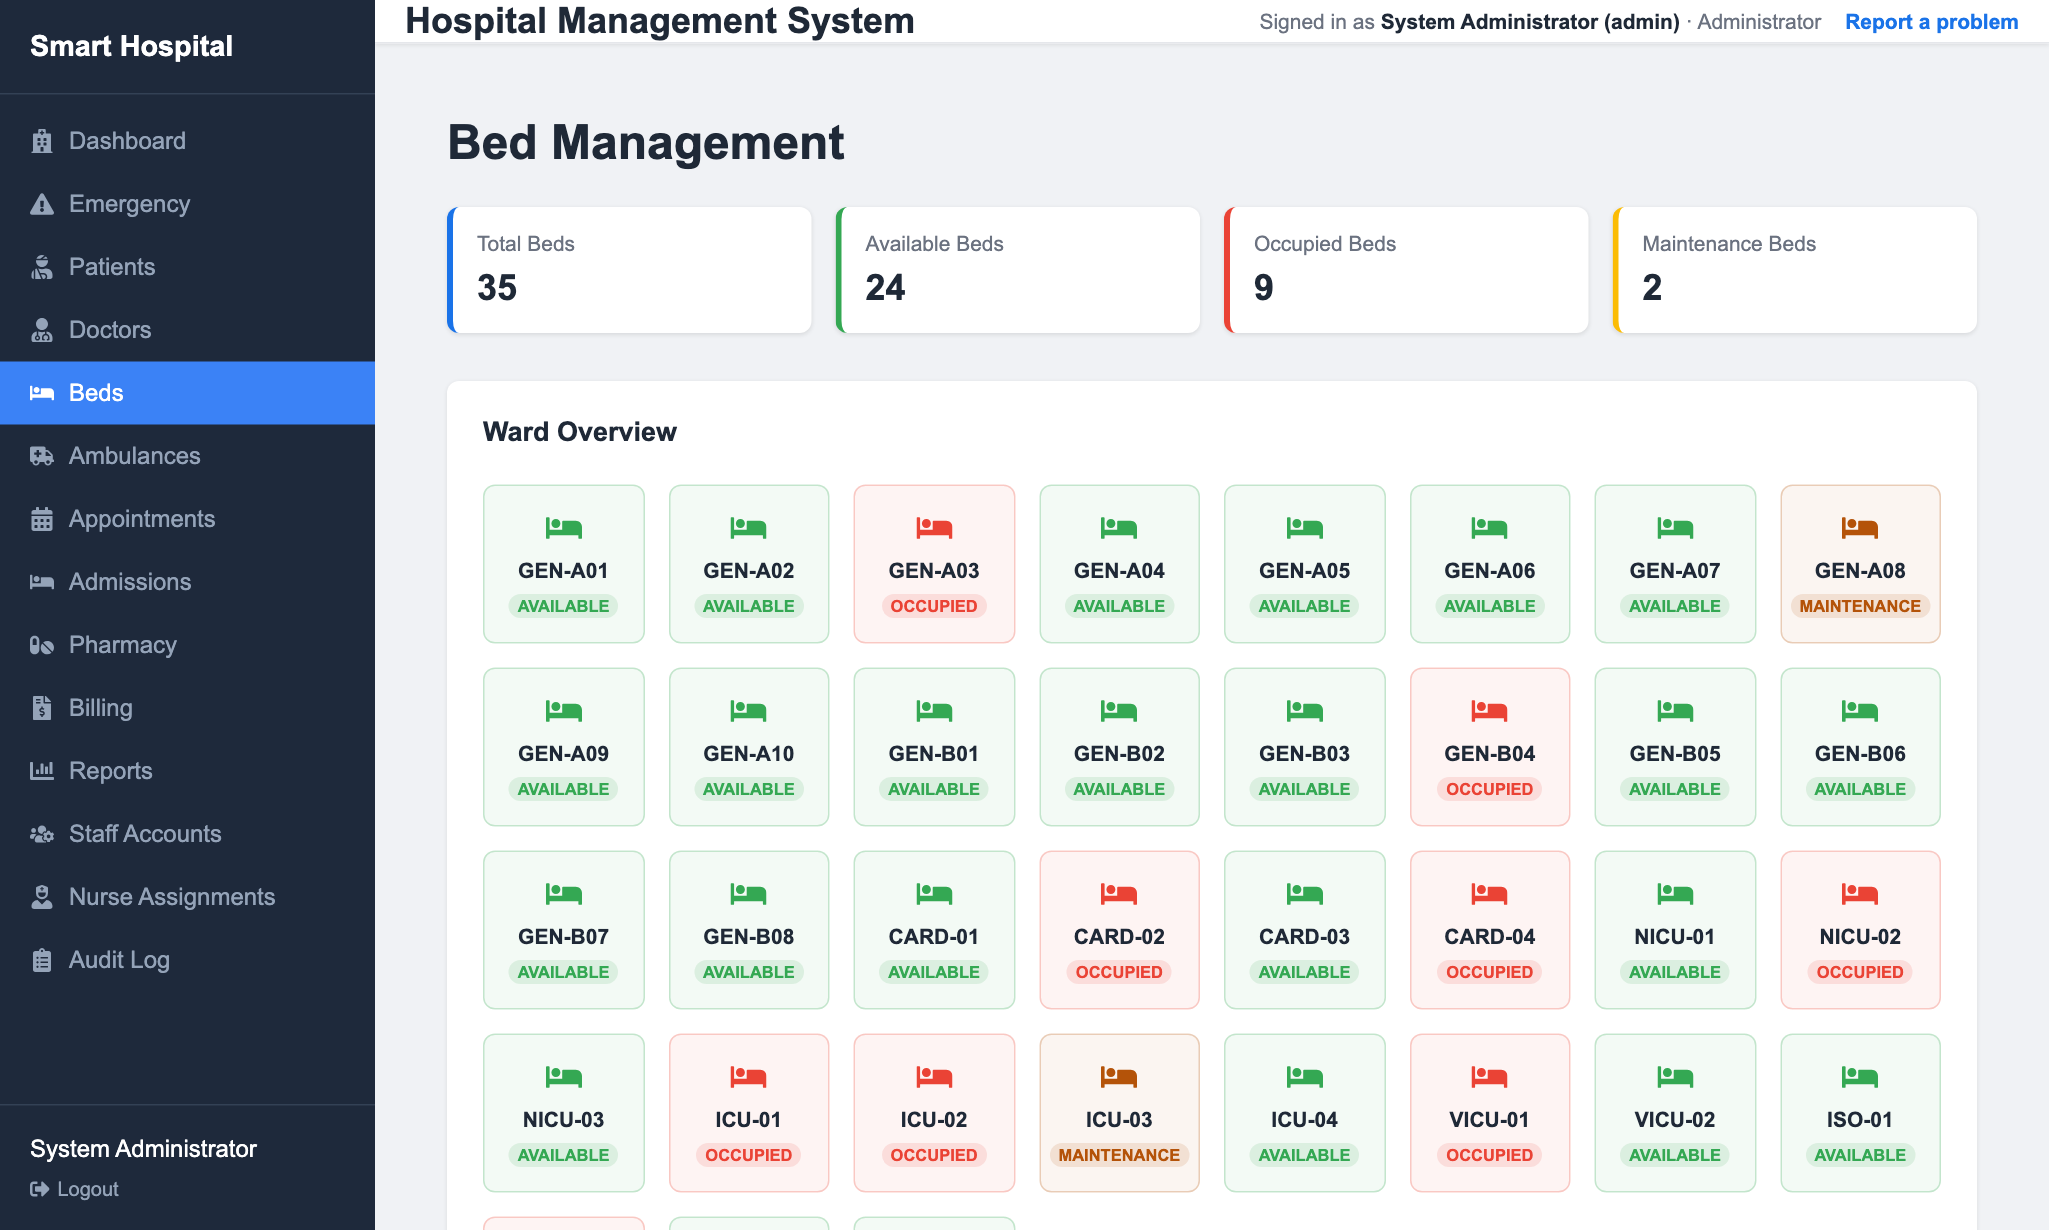
\includegraphics[width=0.485\textwidth]{admin-beds.png} & 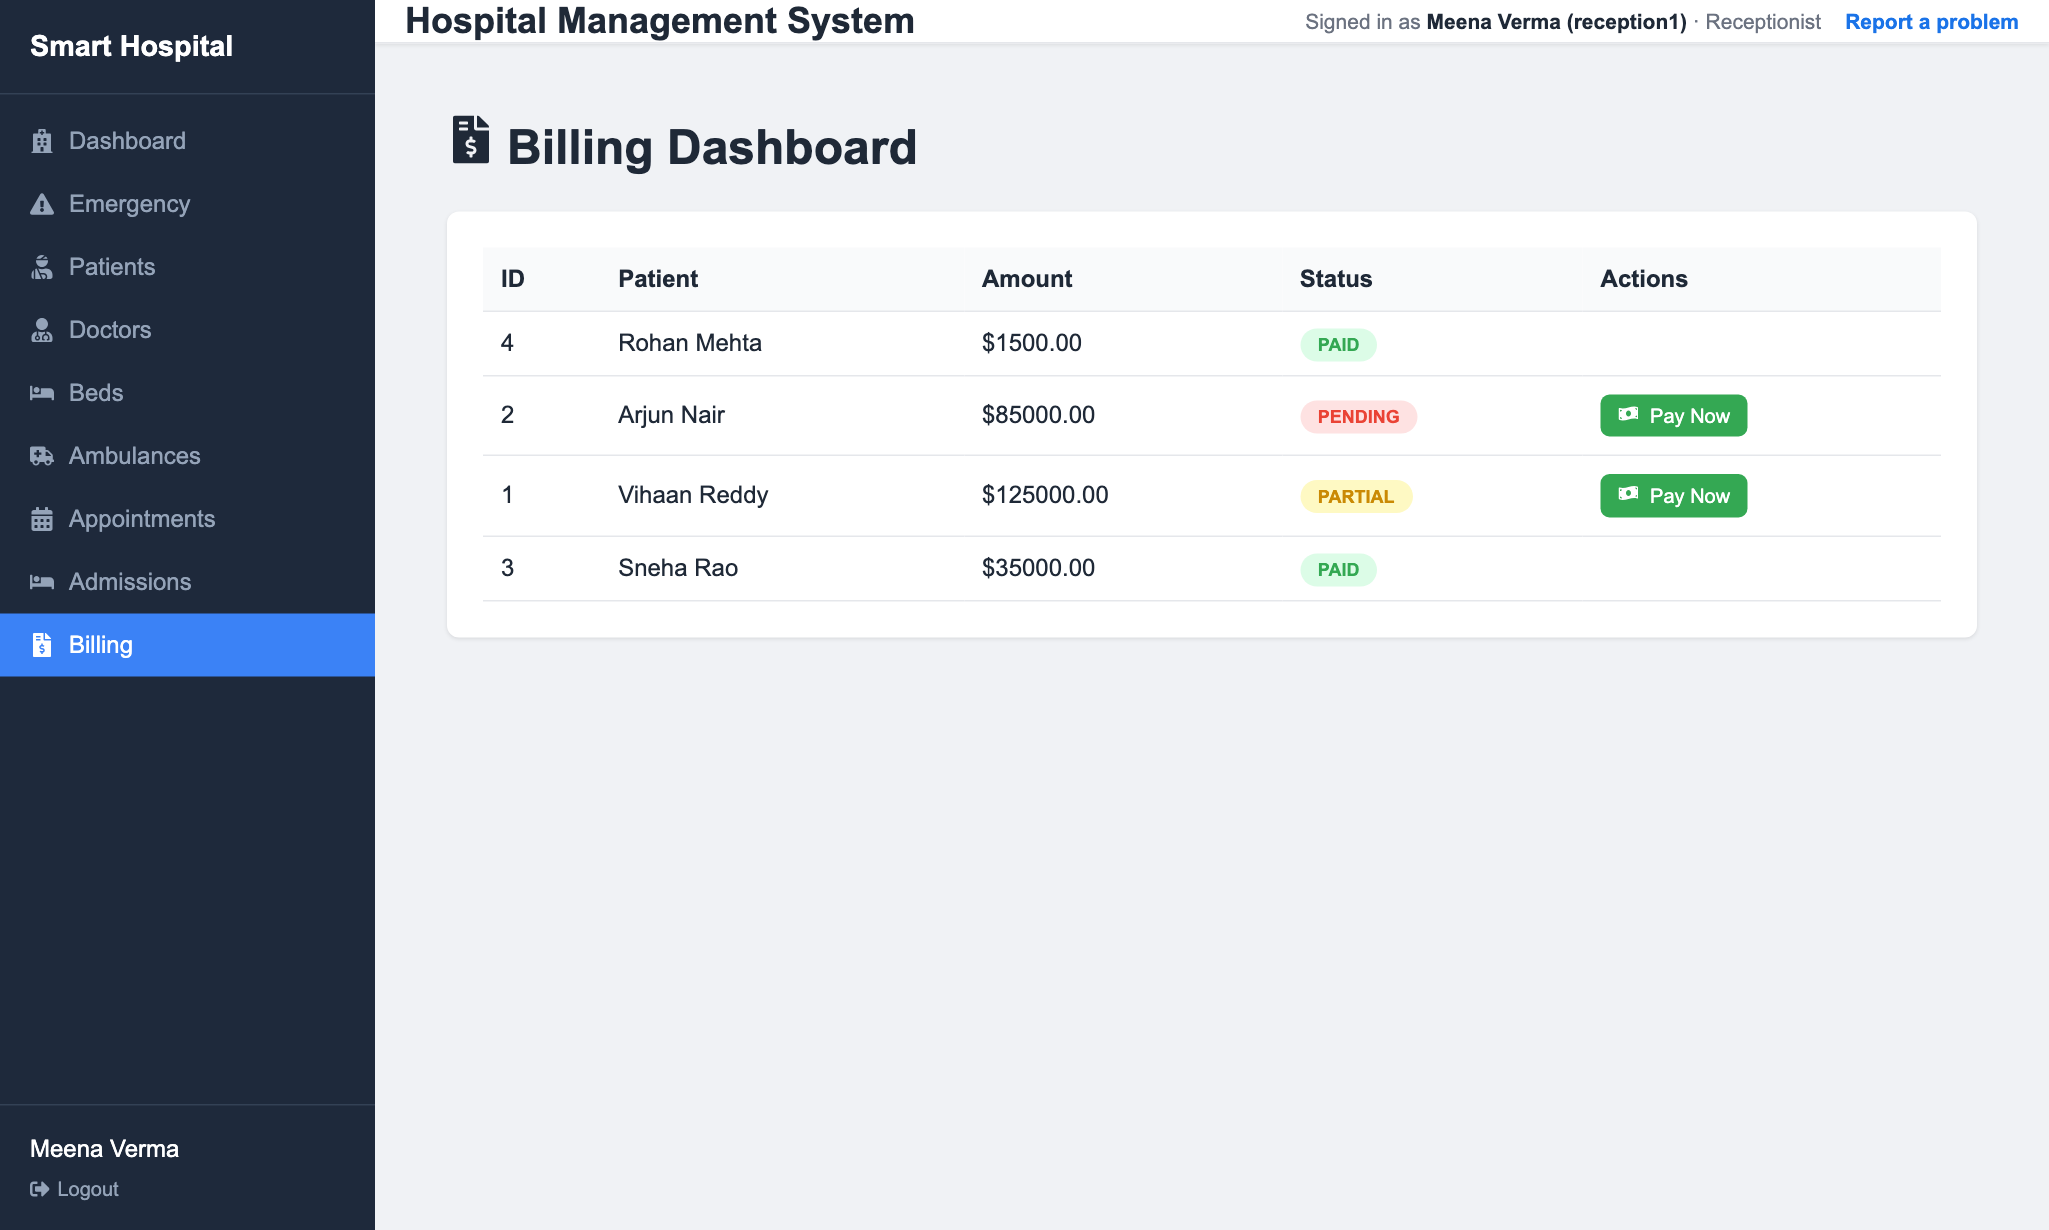
\includegraphics[width=0.485\textwidth]{reception-billing.png} \\
\small (e) Bed board & \small (f) Receptionist: billing \\
\end{tabular}
\caption{Further screens (test data)}\label{fig:more-screens}
\end{figure}

\chapter{Team Contribution}
\begin{tabularx}{\textwidth}{@{}p{4cm}p{3cm}X@{}}
\toprule
\textbf{Team member} & \textbf{Roll number} & \textbf{Contribution} \\\midrule
\placeholder{name} & \placeholder{roll no.} & \placeholder{contribution} \\[8pt]
\placeholder{name} & \placeholder{roll no.} & \placeholder{contribution} \\[8pt]
\placeholder{name} & \placeholder{roll no.} & \placeholder{contribution} \\[8pt]
\placeholder{name} & \placeholder{roll no.} & \placeholder{contribution} \\
\bottomrule
\end{tabularx}

\chapter*{Suggested Evaluation Scheme}
\addcontentsline{toc}{chapter}{Suggested Evaluation Scheme}
\begin{center}
\begin{tabular}{@{}lrl@{}}
\toprule
\textbf{Component} & \textbf{Marks} & \textbf{Where in this report} \\\midrule
Problem analysis and requirements & 5 & Chapters 1, 2 \\
ER diagram and constraints & 10 & Chapter 3 \\
ER-to-relational mapping & 10 & Chapter 4 \\
Functional dependencies and keys & 10 & Chapter 5 \\
Normalization & 15 & Chapter 6 \\
MySQL schema, constraints, and sample data & 10 & Chapters 7, 8.1--8.5, Appendix A \\
SQL queries and advanced DBMS features & 15 & Sections 8.6, 8.7 \\
Front-end integration and functionality & 10 & Chapter 9 \\
Testing and report quality & 5 & Chapter 10 \\
Viva and conceptual understanding & 10 & -- \\\midrule
\textbf{Total} & \textbf{100} & \\
\bottomrule
\end{tabular}
\end{center}
\textbf{Evaluation principle:} Marks should primarily reflect the correctness of database design, ER-to-relational
mapping, functional dependencies, normalization, SQL implementation, and understanding of DBMS concepts. Front-end
appearance alone must not determine the project grade.
